\subsection{Prism design}
\label{prism}
The figure \ref{fig:prism} on page \ref{fig:prism} gives a overview of the receiver optics. After the receiver's second parabolic mirror, the prism is used to filter out all the noisy light except wavelength at 472[nm] to 474[nm]. The prism needs to be accuracy enough to perform the filtering in limited distance. The design contains the type of prism glass material, the incident angle($\alpha$) and prism apex angle($A$).

\begin{figure}[ht!]
\centering
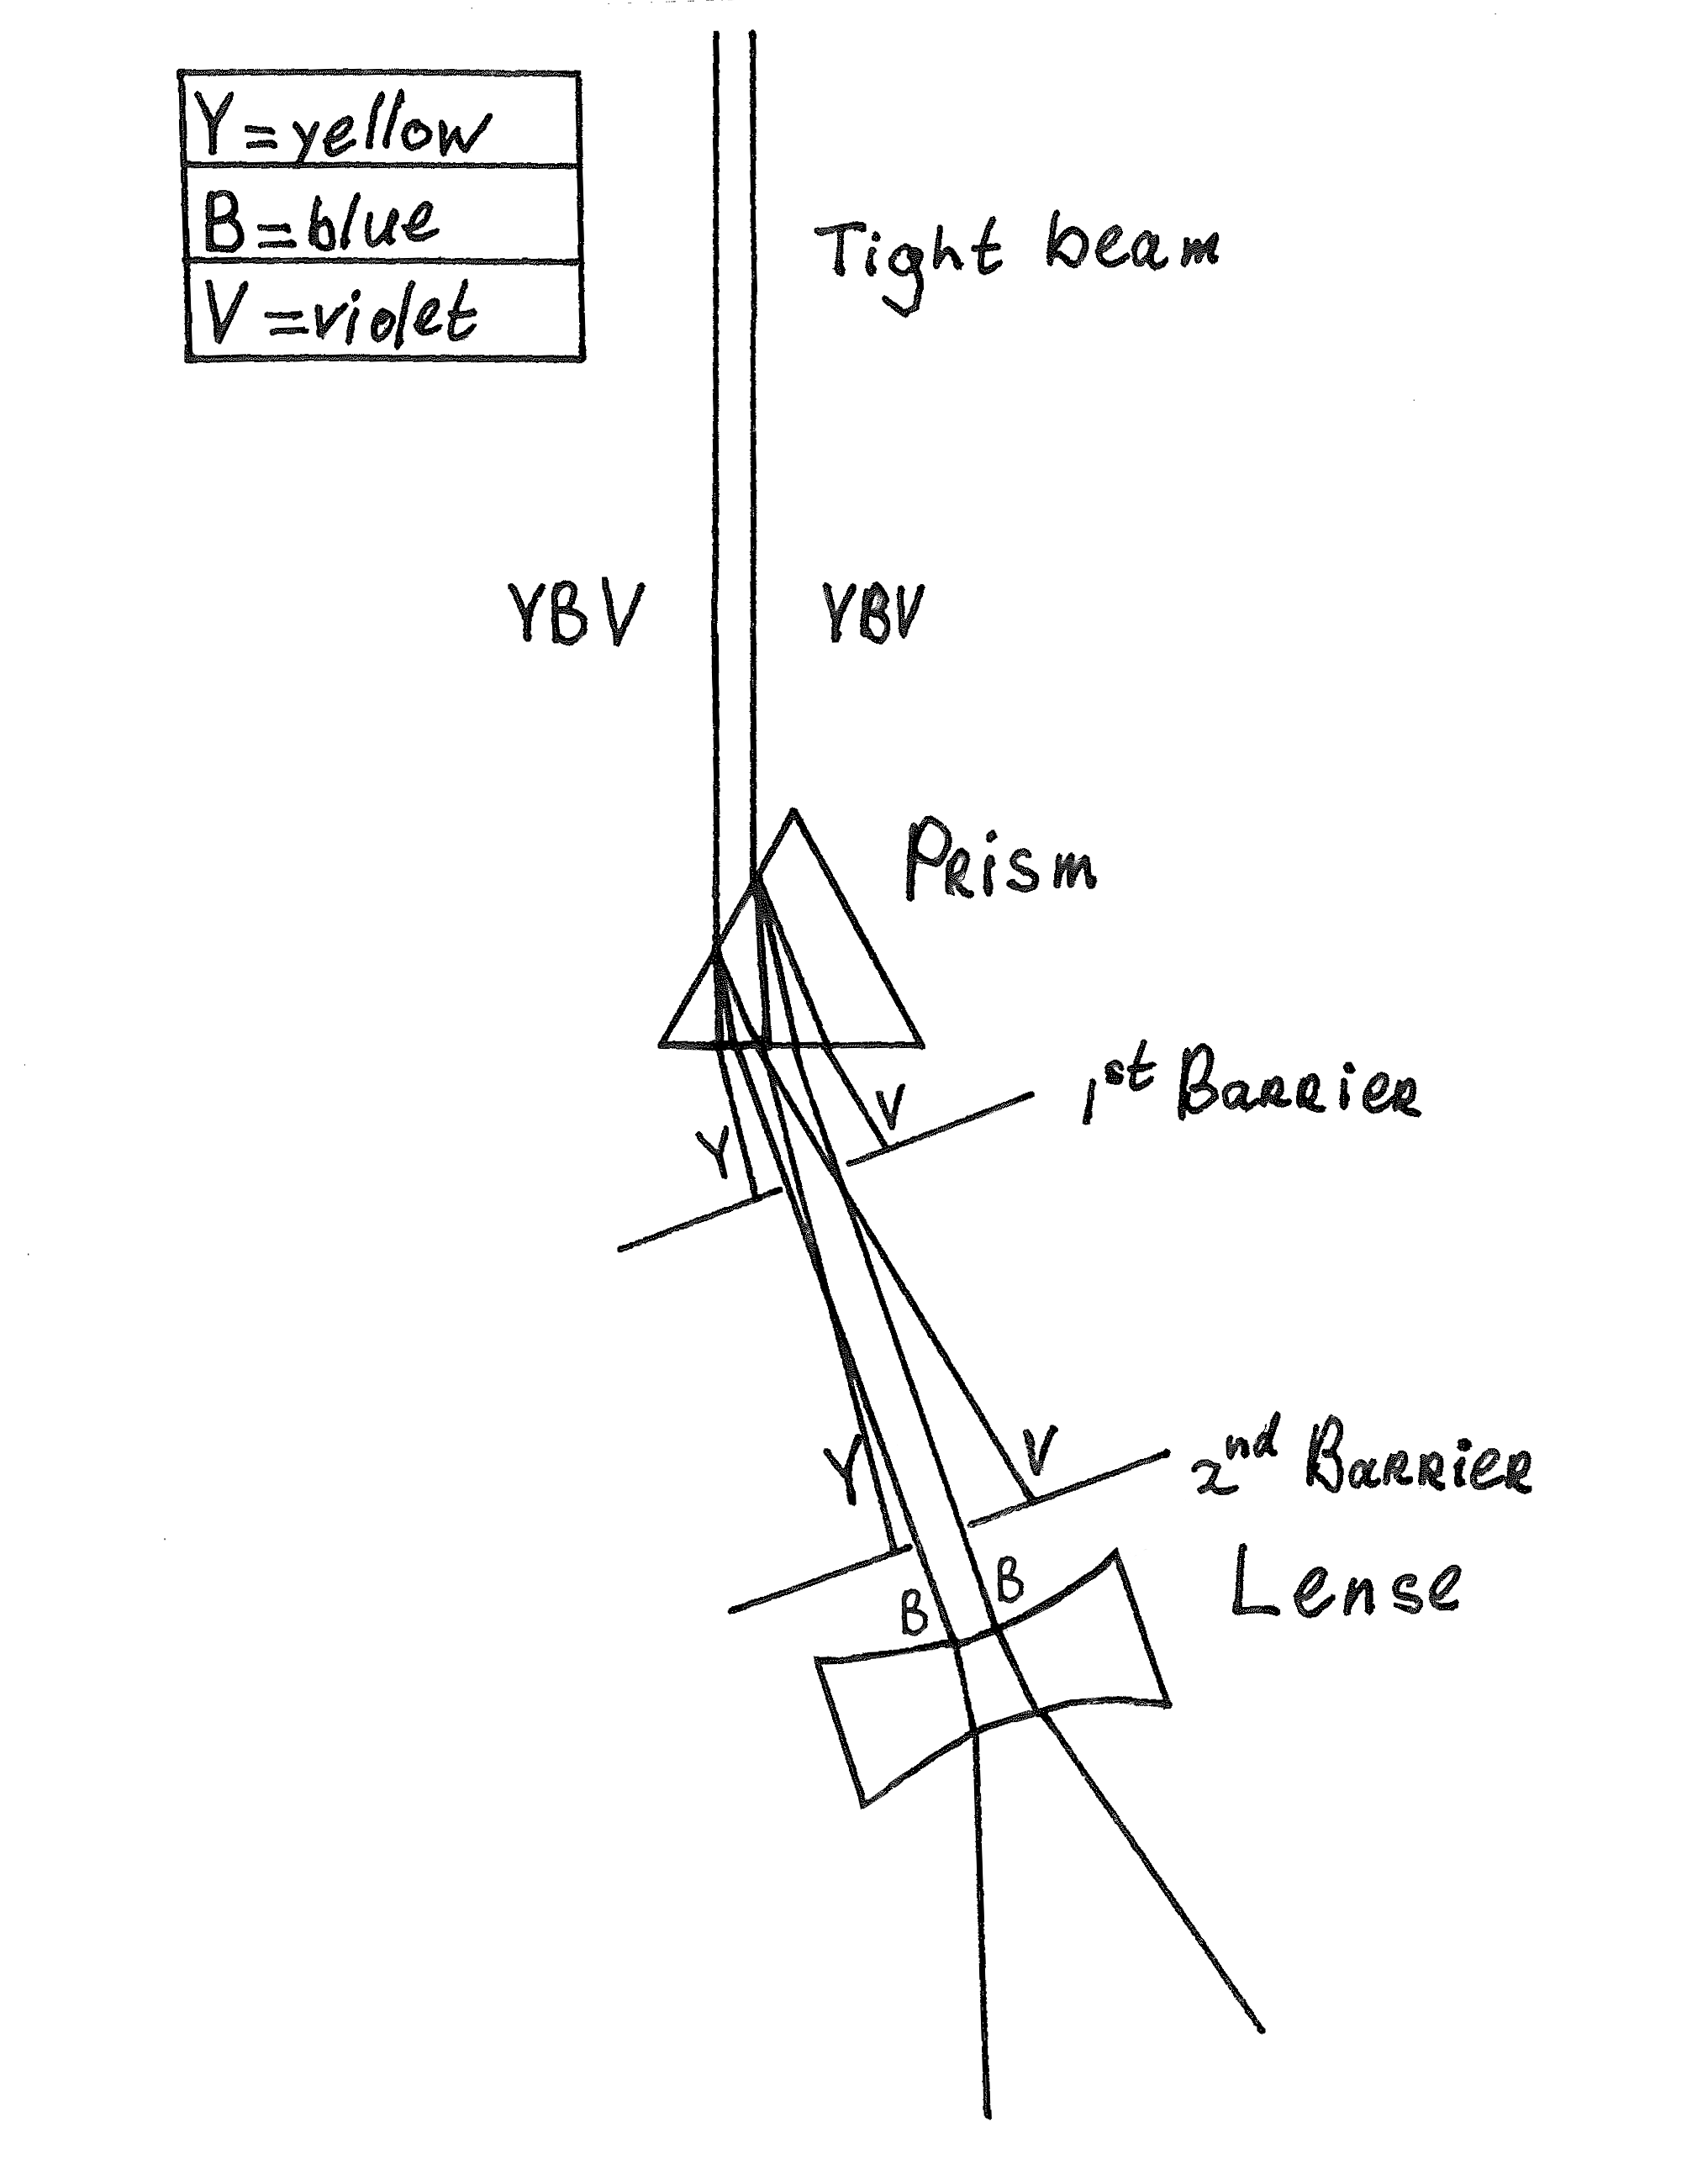
\includegraphics[scale = 0.8]{chapters/img/Prism.png}
\caption{Receiver optics overview}
\label{fig:prism}
\end{figure} 


\begin{figure}[ht!]
\centering
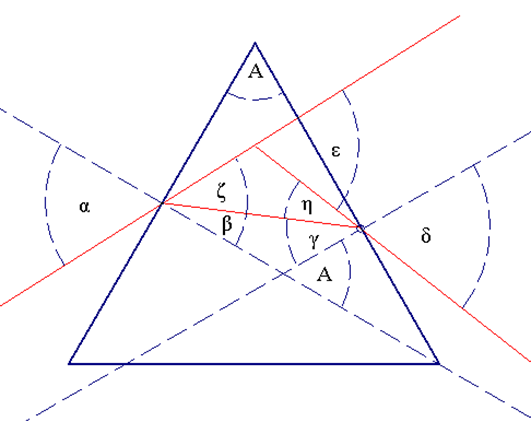
\includegraphics[scale = 1]{chapters/img/Prism2D.png}
\caption{Prism angles define in 2D}
\label{fig:prism2D}
\end{figure} 

In figure \ref{fig:prism2D} on page \ref{fig:prism2D}, the deviation angle $\epsilon$ can be calculated using the formula\cite{prism_angle_calculation}:
\begin{equation}
\label{epsilon}
\epsilon = \alpha - A + sin^{-1}(sin(A)\sqrt{n^2 - (sin(\alpha))^2} - cos(A)sin(\alpha))
\end {equation}
The key requirement to design the prism is to maximize the $\frac{d\epsilon}{d\lambda}$,  because for wavelength 473[nm] larger $\frac{d\epsilon}{d\lambda}$ leads to smaller distance between prism and barriers as well as smaller size of the barrier. The equation \ref{epsilon} shows that the deviation angle($\epsilon$) is a function of A, $\alpha$ and n. From Sellmeier formula\cite{prism_book}, the index of refraction n can be calculated as:
\begin{equation}
\label{index_refraction}
n^2 - 1 = \frac{a_{1}\lambda^2}{\lambda^2-b_{1}} + \frac{a_{2}\lambda^2}{\lambda^2-b_{2}} + \frac{a_{3}\lambda^2}{\lambda^2-b_{3}}
\end {equation}
In the equation \ref{index_refraction}, $a_{1}, a_{2}, a_{3}$ and $b_{1}, b_{2}, b_{3}$ are the dispersion coefficients, which have different values for different glasses. In this case, the most 17 common prism glasses from Schott\cite{prism_material}\cite{prism_book} company are analyzed. Since it is difficult to calculate $\frac{d\epsilon}{d\lambda}$ analytically, $\Delta\epsilon$ due to wavelength 472[nm], 473[nm] and 474[nm] can be obtained by inserting arbitrary A and $\alpha$, which is actually the $\frac{d\epsilon}{d\lambda}$ since the wavelength difference is only 1[nm] of each. During the calculation, no matter what values are given to A and $\alpha$, SF11 glass always has the maximum value of $\Delta\epsilon$ which means it is the optimal glass material. Meanwhile, SF11 glass also has an internal transmittance of 97\% for wavelength around 473[nm], which is acceptable. Next step is to determine the prism apex angle(A) and the incident angle($\alpha$). The prism apex angle is defined as 60 degrees because which gives the most average value for $\Delta\epsilon$. Meanwhile, this kind of euqilateral prisms are also referred to as dispersing prisms used for wavelength separating applications(see figure \ref{fig:prism_equilateral} on page \ref{fig:prism_equilateral}). 

\begin{figure}[ht!]
\centering
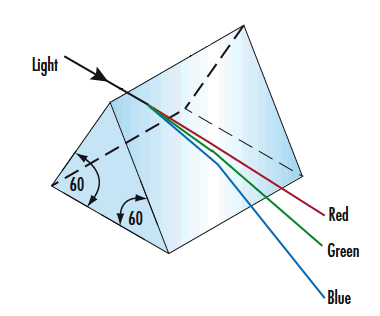
\includegraphics[scale = 0.8]{chapters/img/prism_equilateral.png}
\caption{Equilateral prism for wavelength separating applications}
\label{fig:prism_equilateral}
\end{figure}

To select the correct incident angle, the figure \ref{fig:prism_alpha} on page \ref{fig:prism_alpha} is used. In the figure, the blue line has the asymptote about $\alpha = 54[deg]$. To avoid the asymptote, $\alpha = 55[deg]$ is selected as the incident angle, which leads to $\epsilon = 76[deg]$ and $\Delta\epsilon = 2.1432[mrad]$. The figure \ref{fig:SF11} is the calculation in the excel sheet. There are two $\Delta\epsilon$ in the calculation, and $\Delta\epsilon1 = \epsilon(472[nm]) - \epsilon(473[nm])$ meanwhile $\Delta\epsilon2 = \epsilon(473[nm]) - \epsilon(474[nm])$. The driving $\Delta\epsilon$ is the smaller one, since it is the minimum requirement. Taking $\Delta\epsilon = 2.1432[mrad]$ into further calculation, in order to separate wavelength 472[nm], 473[nm] and 474[nm], barrier radius(or beam width) 1[mm] leads to distance 0.4666[m] between prism and barrier. To short the distance, more concentrated beam is needed from parabolic mirror. The figure \ref{fig:prism_final} on page \ref{fig:prism_final} shows the final values of all angles.

\begin{figure}[ht!]
\centering
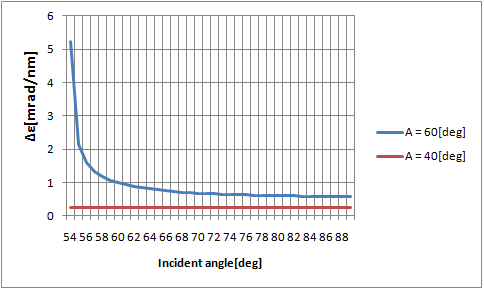
\includegraphics[scale = 1.2]{chapters/img/prism_alpha.png}
\caption{Plot of $\Delta\epsilon$ due to different incident angles}
\label{fig:prism_alpha}
\end{figure}

\begin{figure}[ht!]
\centering
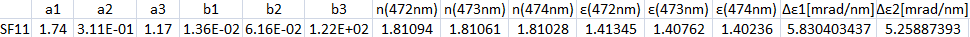
\includegraphics[scale = 0.8]{chapters/img/SF11.png}
\caption{Glass 'SF11' calculations}
\label{fig:SF11}
\end{figure}

\begin{figure}[ht!]
\centering
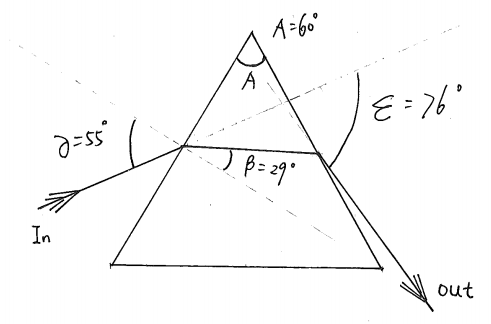
\includegraphics[scale = 0.8]{chapters/img/prism_final.png}
\caption{Overview of all angles}
\label{fig:prism_final}
\end{figure}